
%%%Präambel%%%
%!TEX program = lualatex
\documentclass[parskip=half]{scrartcl}
%%%Präambel zum laden benötigter Packages%%%

%Anpassung des Dokuments auf die deutsche Sprache
\usepackage[ngerman]{babel}

%Links und Verweise innerhalb des Dokuments erzeugen

\usepackage[breaklinks, pdftex]{hyperref}

%Geometrische Form des Dokuments
\usepackage[a4paper, left=3cm, right=2cm, top=3.5cm , bottom=2.5cm]{geometry}

%Paket zum einbinden von Bildern und Grafiken
\usepackage{graphicx}

%Für zwei Bilder nebeneinander
\usepackage{subfigure}

%Matheumgebung
\usepackage{amsmath}

%Mathematische Symbole
\usepackage{amssymb}

%Transformationszeichen
\usepackage{trfsigns}

%Fancy-Mathe-Buchstaben (z.B. Laplace L)
\usepackage{mathrsfs}

%Paket zum Darstellen von SI-Einheiten
\usepackage{siunitx}

%Sourcecode Printer in Latex
\usepackage{listings}

%Paket zum einbinden von Tikz-Dateien(Matlab)
\usepackage{pgfplots}
\pgfplotsset{compat=1.16}


%Ausgabeformat der PDF
\usepackage[T1]{fontenc}

%Eingabeformat der Latex Datei
\usepackage[utf8]{inputenc}

%Horizontale Linien innerhalb einer Tabelle
\usepackage{booktabs}

%Tabelle mit festen Breiten 
\usepackage{tabularx}

\usepackage{csquotes}
 
%Zeilenabstand einstellen 
\usepackage[onehalfspacing]{setspace}
%Befehle zum umschalten des Zeilenabstandes 
%\onehalfspacing             % anderthablfacher Zeilenabstand 

%Absatzabstand einstellen
\setlength{\parskip}{6pt}
%Absatzeinzug einstellen
\setlength{\parindent}{0pt}

%Erstellen von Abkürzungen+ Verzeichnis
\usepackage[withpage]{acronym}
%Optionen:	footnote: Fußnoten der kurzform
%			nohyperlinks: keine Verlinkungen
%			printonlyused: nur verwendete Abkürzungen
%			smaller: verkeinerung der Anzeige der Abkürzung
%			dua: Langform der Abkürzung angezeigt
%			nolist: Keine Übersciht der Abkürzungen
%			withpage: Gibt die Seitenzahl mit an



%Für den Float Specifier  
\usepackage{float}

		
%Bibliotheksverwaltung und Zitieren
\usepackage[backend=biber,url=false, sorting=none]{biblatex}

%Definition eines Literatur und eines Quellenverzeichnisses
\defbibheading{AL}{\section*{Literatur}}
\defbibheading{QL}{\section*{Quellen}}
\bibliography{Meine_Bibliothek.bib}
\defbibfilter{AL}{\not\keyword{Quellen}}
\defbibfilter{QL}{\keyword{Quellen}} %Quellen benötigen das Keyword "Quellen" in Jabref!
%Änderung in Buchstaben mit dem Feld "Shorthand"!
%Entfernen der Anführungszeichen im Titel und Hinzufügen eines Doppepunktes

\DeclareFieldFormat[article]{title}{{#1}}
\DeclareFieldFormat[misc]{title}{#1}
\DeclareFieldFormat[article]{title}{{#1}}
\DeclareFieldFormat[MastersThesis]{title}{#1}

\DefineBibliographyStrings{german}{% 
        andothers = {{et\,al\adddot}},             
        editor = {(Hrsg.)}, 
        editors = {(Hrsg.)}}
        
   

%Einstellung neue Längen
\newlength\Bildbreite
\setlength\Bildbreite{0.9\textwidth}

\numberwithin{equation}{section} 
\renewcommand{\theequation}{\arabic{section}.\arabic{equation}}


\usepackage[labelfont={bf,sf},font={small},%
  labelsep=space]{caption}

\addbibresource{Meine_Bibliothek.bib} %Bibliographiedateien laden
\begin{document}
%%__Deckblat__t%%

\title{Grundlagen CAN-Bus}
\author{Philipp Flegler, Tomke Wegers}
\date{24. April 1999}

\maketitle
%%_____%%

\newpage
\tableofcontents
\newpage

\section{Einleitung}

    
Die vorliegende Hausarbeit beschäftigt sich mit dem Controller Area Network (CAN) und dessen Telegrammen. Ziel der Arbeit ist es, die Struktur und Funktionsweise von CAN-Telegrammen zu erläutern und die verschiedenen Aspekte des CAN-Bussystems zu untersuchen. Die Arbeit beginnt mit einer detaillierten Beschreibung der beiden grundlegenden Telegrammtypen: den Standard-CAN-Frames nach der Spezifikation 2.0A und den Extended-CAN-Frames nach der Spezifikation 2.0B. Hierbei wird insbesondere auf den Unterschied in der Länge des CAN-Identifiers und der verfügbaren logischen Adressen eingegangen.

Anschließend wird der Buszugriffsmechanismus im CAN-Bus behandelt, wobei der Ablauf der bitweisen Arbitrierung und die Bedeutung der Priorität der Nachrichten thematisiert werden. Ein weiterer wichtiger Bestandteil der Arbeit ist das Fehlermanagement im CAN-System. Hierzu werden die verschiedenen Fehlerarten und die Funktionsweise der Fehlererkennung sowie die Maßnahmen zur Fehlerbehandlung erläutert.

Abschließend wird das CAN-Protokoll im Kontext des ISO/OSI-Modells betrachtet, wobei der Fokus auf der physikalischen und der Sicherungsschicht liegt. Diese Struktur ermöglicht es, die Funktionsweise des CAN-Bussystems in einem größeren Netzwerkzusammenhang zu verstehen. Die Arbeit ist in mehrere Abschnitte unterteilt, die aufeinander aufbauen und die relevanten Themen des CAN-Busses detailliert darstellen.


\section{CAN-Telegramme}

    Es gibt zwei unterschiedliche Arten von CAN-Telegrammen: die Standard-CAN-Frames (kurze Telegramme nach CAN-Spezifikation 2.0A) und die Extended-CAN-Frames (lange Telegramme nach CAN-Spezifikation 2.0B). Der wesentliche Unterschied zwischen diesen beiden Telegrammarten liegt in der Länge des CAN-Identifiers bzw. in der Anzahl der verfügbaren logischen Adressen. Beim Telegramm nach CAN-Spezifikation 2.0A ist der Identifier 11 Bits lang, sodass 2048 verschiedene logische Adressen möglich sind. Beim Telegramm nach CAN-Spezifikation 2.0B beträgt die Länge des Identifiers 29 Bits, was 536.870.912 logische Adressen ermöglicht. \cite{lawrenzCANControllerArea2016}

\subsection{Aufbau von kurzen CAN-Telegrammen}
Im folgenden Abschnitt wird zunächst der Aufbau eines kurzen Telegramms beschrieben, bevor im Anschluss auf die Besonderheiten des langen Telegramms eingegangen wird. Ein CAN-Telegramm lässt sich in unterschiedliche Abschnitte bzw. Felder unterteilen. 

    \begin{figure}[htbp]
    \centering
    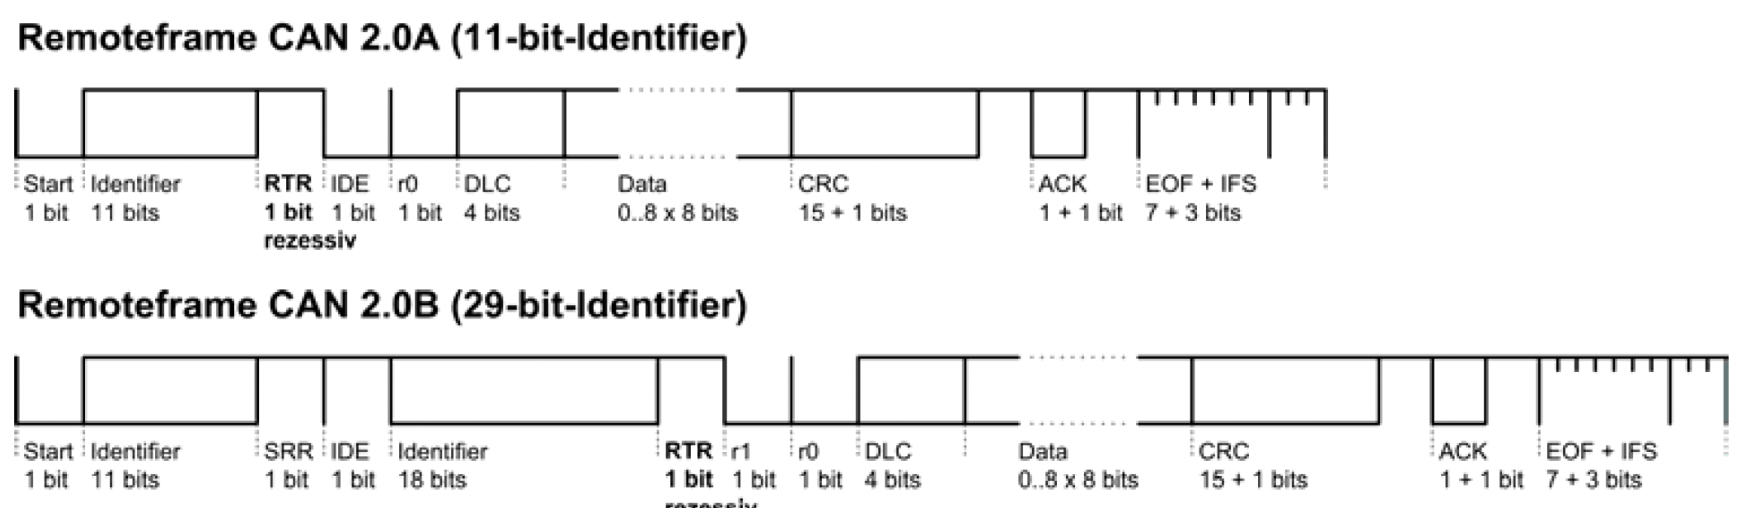
\includegraphics[width=\Bildbreite]{Grafiken/CAN_Telegrame-crop.pdf}
    \caption{CAN-Telegramme \cite{lawrenzCANControllerArea2016}}
    \label{fig: CAN_Telegramme}
    \end{figure}    

Der erste Abschnitt ist das Arbitration-Feld, das zur Regelung des Buszugriffs benötigt wird (siehe Abbildung \ref{fig: CAN_Telegramme}).
Das Arbitration-Feld beginnt mit einem Startbit, das immer "low" (dominant) ist. Auf das Startbit folgt der 11 Bit lange Identifier, der den Inhalt und die Priorität des Telegramms enthält. Je höher der Wert des Identifiers, desto niedriger ist die Priorität des Telegramms. Das letzte Bit im Arbitration-Feld ist das Remote Transmission Request-Bit (RTR-Bit), welches angibt, ob das Telegramm Daten enthält oder ob der entsprechende Teilnehmer aufgefordert wird, ein Telegramm zu senden.

Auf das Arbitration-Feld folgt das Control-Feld. Dieses beginnt mit dem Identifier Extension Bit (IDE-Bit), das bei Standard-Frames auf "low" (dominant) gesetzt ist. Das folgende r0-Bit ist reserviert. Im 4 Bit langen DLC-Bereich des Control-Feldes ist die Länge der nachfolgenden Daten festgelegt.

Das darauf folgende Data-Feld kann 0 bis 8 Byte lang sein und enthält die eigentlichen Nutzdaten des Telegramms.

Nach dem Data-Feld folgt das 16 Bit lange CRC-Feld, welches zur Fehlererkennung dient. Durch das CRC-Feld können Einzelbitfehler bis zu einer Anzahl von 6 und aufeinanderfolgende Bitfehler (Burst-Errors) bis zu einer Länge von 15 Bit erkannt werden. Eine genauere Ausführung zur Fehlererkennung erfolgt im Kapitel Fehlermanagement.

Nach dem CRC-Feld folgt das ACK-Feld mit einer Länge von 2 Bit. Die Busteilnehmer, die eine gesendete Nachricht korrekt empfangen haben, bestätigen dies, indem sie einen dominanten Pegel auf dem ersten Bit des ACK-Feldes senden. Der Sender der Nachricht interpretiert einen nicht-dominanten Pegel als Fehler. Das letzte Bit im ACK-Feld ist der ACK-Delimiter, der immer rezessiv ist.

Das letzte Feld ist das EOF-Feld (End-Of-Frame-Feld), das mit einer Länge von 7 Bit das Ende des Telegramms markiert. Im EOF-Feld sind alle Bits rezessiv.

Um den Busteilnehmern nach einem Telegramm Zeit zum Abspeichern des Telegramms zu geben, folgt der sogenannte Interframe Space (IFS) mit einer Länge von 3 Bit. Auch hier sind alle Bits rezessiv.

Durch die aufeinander folgenden rezessiven Bits wird signalisiert, dass der Bus aktuell nicht genutzt wird. Ein neuer Teilnehmer kann dann durch ein Startbit ein neues Telegramm senden.

\subsection{Besonderheiten von langen CAN-Telegrammen}
Wie in Abbildung \ref{fig: CAN_Telegramme} zu sehen, folgt bei einem langen Datentelegramm nach den ersten 11 Bits des Identifiers ein SRR-Bit (Substitute Remote Request) anstelle des RTR-Bits bei kurzen Telegrammen. Das darauf folgende IDE-Bit liegt bei langen Telegrammen an derselben Stelle wie im kurzen Telegramm. Jedoch ist dieses IDE-Bit im langen Telegramm rezessiv und kündigt damit an, dass weitere 18 Identifier-Bits folgen. Nach diesen Bits ist der Identifier im Extended-CAN-Frame vollständig, und danach folgt ein RTR-Bit mit derselben Funktion wie im kurzen Telegramm.

Auf das RTR-Bit folgt im langen Telegramm das 6 Bit lange Control-Feld, in dem die ersten zwei Bits, r0 und r1, reserviert sind. Auf diese folgen 4 Bits, die die Längeninformation der darauffolgenden Daten enthalten.










\section{Buszugriff}
Das CAN-Bussystem ist ein Multi-Master-System mit mehreren Busteilnehmern. 
Daher muss der Zugriff auf den Bus geregelt werden, um zu verhindern, 
dass der Bus dauerhaft besetzt ist. 
Hierfür regelt das CAN-Bussystem den Zugriff mithilfe der zerstörungsfreien, bitweisen Arbitrierung.

Wie oben erläutert, befindet sich in jedem CAN-Telegramm ein Arbitrierungsfeld, das aus dem Startbit, 
einem Identifier und einem RTR-Bit (Remote Transmission Request) besteht. 
Für den Buszugriff sind jedoch nur das Startbit und der Identifier relevant, da diese die Priorität 
der Nachricht festlegen. Dabei gilt: Eine Null ist dominant, und eine Eins ist rezessiv. 
Das RTR-Bit wird nur dann genutzt, wenn ein Teilnehmer Daten von einem anderen Teilnehmer anfordert.

Die Priorität der Nachricht wird durch die Wertigkeit des Identifiers bestimmt. 
Nachrichten mit kleineren Identifiern haben höhere Priorität und setzen sich bei gleichzeitigem 
Zugriff auf den Bus durch. Da der CAN-Bus durch eine Null in einem Bit als „dominant“ belegt wird, 
führt ein niedrigerer Identifier (mit mehr Nullen) automatisch zu einer höheren Priorität.

\subsection{Ablauf der Arbitrierung}
Wenn zwei oder mehr Teilnehmer gleichzeitig auf den Bus zugreifen, 
folgt der Zugriff einem klaren Ablauf: Beide Teilnehmer senden zunächst ihr 
Startbit (z. B. 0 = dominant), wodurch der Bus auf den dominanten Zustand eingestellt wird. 
Beide Teilnehmer lesen den Zustand aus und senden weiter, solange die Bits, die sie senden, 
mit dem empfangenen Wert übereinstimmen. Auf diese Weise erkennen sie nicht, 
dass ein anderer Teilnehmer ebenfalls sendet.

Dieser Prozess der bitweisen Arbitrierung setzt sich fort, bis es zu einer Abweichung in den 
gesendeten Bits kommt. In diesem Moment stellt der Teilnehmer, der eine Eins (rezessiv) gesendet hat, 
fest, dass sein Signal vom anderen Teilnehmer (der eine Null gesendet hat) „überstimmt“ wurde. 
Der Teilnehmer mit dem rezessiven Bit bricht daraufhin die Übertragung ab und schaltet in den 
Empfangsmodus, während der Teilnehmer mit dem dominanten Bit seine Nachricht ohne Unterbrechung 
weitersendet.

Dieses Verfahren wird als „zerstörungsfrei“ bezeichnet, 
da der Teilnehmer mit der höheren Priorität (der das dominante Signal gesendet hat) seine 
Übertragung nicht neu starten muss. Der abgebrochene Teilnehmer bleibt im Empfangsmodus und 
kann die Nachricht weiterhin lesen, da sie auch für ihn relevant sein könnte. 
Er muss das Telegramm nicht neu starten, da es den gleichen Anfang hat wie seine eigene Nachricht.

\subsection{Sicherheit und Fehlertoleranz}
Diese bitweise Arbitrierung macht das CAN-Bussystem besonders sicher und fehlertolerant. 
Da die Arbitrierung zerstörungsfrei erfolgt, gehen keine Daten verloren, 
und konkurrierende Teilnehmer können ihre Nachrichten sofort erneut senden, 
sobald der Bus wieder frei ist. Dadurch wird eine hohe Datenintegrität und Effizienz gewährleistet.

\subsection{Physikalische Einstellung des Buszustands}
Voraussetzung für dieses System ist die richtige Einstellung des physikalischen Treibers, 
sodass 0 als dominant und 1 als rezessiv erkannt wird. 
In den meisten standardisierten CAN-CPUs ist die Null als dominant eingestellt, 
sodass Nachrichten mit kleineren Identifiern (mehr Null-Bits) automatisch eine höhere 
Priorität haben.

\section{Fehlermanagment}

    
\subsection{Arten von Fehlern}
Ein Bussystem sendet eine große Menge an Daten, dabei kann es zu Fehlern in der Übertragung kommen.
Der CAN benutzt hierfür das "Data Link Layer" welches in standardisierten CAN-Chips implementiert ist.
Es gibt verschiedene Fehler diese werden folgend aufgeführt:
Bit Fehler: Bei der Überprüfung der Nachricht gibt es einen Falschen Wert.

Bit-Stuffing-Fehler: In CAN wird eine Bitfolge von mehr als 5 gleichen Bits als Fehler erkannt.

Es sei den es handelt sich um das EOF (End of Frame)

Fehler: Die CRC-Prüfsumme stimmt nicht mit der berechneten übereinstimmen.

Format Fehler: Es liegt das falsche Datenformat vor.

Acknowledgement Fehler: Ein Sender empfängt von keinem Busteilnehmer ein dominates Bit im Acknowledgement
-Slot
\subsection{Funktionsweise des Fehlermanagment}
Der CAN behandelt Fehler immer nach dem gleichen Prinzip dieses wird im folgenden aufgeführt.
Zunächst muss einer der oben genannten Fehler genannt werden dafür sind diese Fehler bei jedem Busteilnehmer
hinterlegt. Nachdem ein Busteilnehmer einen Fehler erkennt hat, sendet er einen Error Frame (mehr als
5 gleiche Bits) das die Stuffing-Regel verletzt. Dies dient zur Übermittlung eines Fehlers an alle anderen
Busteilnehmer, dadurch verwerfen alle Busteilnehmer das zuvor empfangene Telegramm. Anschließend
werden bei den Busteilnehmern die Zähler TEC(Transmission Error Counter) oder REC(Receive Error Counter)
beeinflusst. Abschließend wird das Telegramm erneut gesendet.
Die oben genannten Zähler dienen dazu um dauerhafte Fehler durch defekte Hard- oder Software zu 
verhindern.
Jeder Busteilnehmer/Knoten kann drei Zustände annehmen je nachdem welchen Wert die Zähler haben.
Diese Zustände bestimmen welche Priorität eines Busteilnehmers hat und zu bestimmen ob ein Busteilnehmer
Fehlermeldungen senden darf oder nicht.
Der erste Zustand ist "Active Error"(TEC \& REC < 128), dieser berechtigt einen CAN-Knoten ein dominantes
Error Frame zu senden sollte er einen Fehler feststellen.
Der zweite Zustand ist "Passive Error"(TEC || REC >127), dieser sorgt dafür das der CAN-Knoten nur noch
rezessive Error Frames zu senden um zu verhindern das der CAN-Knoten den Bus weiter mit Fehlermeldungen
behindert.
Der letzte Zustand ist "Bus Off"(TEC > 255), dieser trennt den Busteilnehmer von der Kommunikation im
Bussystem. Dieser Zustand kann nur verlassen werden durch einen Soft- oder Hardware Reset.

Wie oben erwähnt werden die Zähler oben beeinflusst, dies geschieht mittels verschiedener Algorithm
um den Fehler beim richtigen Knoten zuzuordnen.


\section{CAN im ISO/OSI-Modell}

    \subsection{Das OSI-Refernezmodell}
Das OSI-Schichtenmodell ist ein Modell zur Veranschaulichung komplexer Kommunikationssysteme.
Komplex bedeutet hierbei, dass sich das Modell mit der Kommunikation zwischen verschiedenen Computersystemen in einem Netzwerk beschäftigt.
Das Modell besteht aus sieben Schichten (auch Ebenen oder Layer genannt), die verschiedene Instanzen enthalten, welche wiederum unterschiedliche Dienste (Services) bereitstellen.

\begin{figure}[htbp]
    \centering
    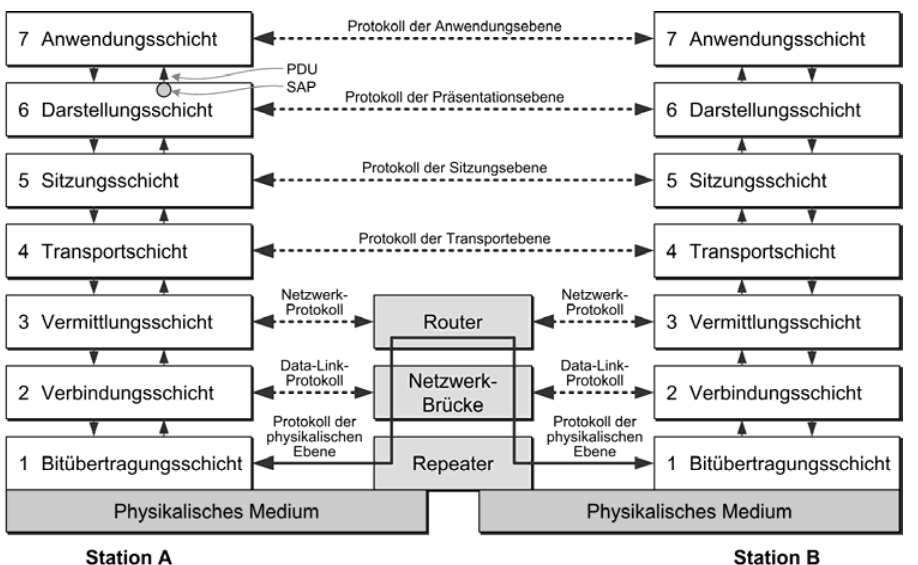
\includegraphics[width=\Bildbreite]{Grafiken/OSI.png}
    \caption{OSI-Modell}
    \label{fig: OSI}
\end{figure} 

Kommunikation zwischen den Schichten
Die Kommunikation der Schichten untereinander erfolgt über sogenannte Dienstzugangspunkte (Service Access Points, SAPs). Dabei ist zu beachten, dass das Ziel darin besteht, dass eine höhere Schicht Daten von den Diensten der darunterliegenden Schichten anfordern oder empfangen kann. Die untere Schicht dient somit als Dienstleister für die obere Schicht.

Um Daten anzufordern oder zu empfangen, werden sogenannte Dienstelemente verwendet. Es ist außerdem wichtig zu wissen, dass eine Schicht mehrere Instanzen und Dienste besitzen kann.

Kommunikation innerhalb einer Schicht
Instanzen innerhalb einer Schicht können über Protokolle miteinander kommunizieren. Dies ermöglicht:

die Bereitstellung eines Dienstes durch die Zusammenarbeit zweier Instanzen, oder
eine effizientere Fehlersuche, da Problemquellen besser isoliert werden können.
Zur Unterscheidung der verschiedenen Dienste werden Service Access Point Identifier (SAPI) verwendet, die bei Anfragen oder beim Empfangen von Daten mit angegeben werden.

Kommunikation zwischen Geräten
Die Kommunikation zwischen zwei Geräten erfolgt über sogenannte PDUs (Protocol Data Units).
Möchte Gerät A Daten an Gerät B senden, erstellt Gerät A in der obersten Schicht eine PDU. Diese PDU wird mit Kontrollinformationen ergänzt und an die nächstuntere Schicht weitergeleitet. Dieser Vorgang wiederholt sich, bis die unterste Schicht erreicht ist.

Die PDU wird dann über das Übertragungsmedium (z. B. Kabel oder Funk) an Gerät B gesendet. Dort wird die PDU von der untersten Schicht entgegengenommen, und jede Schicht überprüft nacheinander die für sie relevanten Kontrollinformationen. Am Ende erhält die oberste Schicht von Gerät B die ursprünglichen Daten.


\subsection{Physikalische Schicht}
CAN-Bus deckt in diesem Modell nur die ersten beiden Schichten ab. CAN deckt die erste Schicht, die physikalische Schicht, ab da ganz klar geregelt ist wie die Übertragung der einzelnen Bits stattfindet. 

\subsection{Sicherungsschicht}
Die zweite Schicht, die Sicherungsschicht wird ebenfalls abgedeckt. Damit diese Schicht abgedeckt wird müssen die Daten in einer klaren Form verpackt werden so das Übertragungsfehler von den Teilnehmenr erkannt werden können. Dies wird im CAN-Bus durch den klaren Aufbau des CAN-Telegrams und das Fehlermanagement gewährleistet.
\section{Zusammenfassung}


\newpage

\section{Literaturverzeichnis}
\printbibliography[title={ }]%hier Bibliographie ausgeben lassen
\newpage
\listoffigures
\end{document}



